\section{Supplementary Material}


\subsection{Experiments}


\subsubsection{Qualitative Comparison}
\begin{figure}[h!]
\tiny{
\begin{verbatim}


CONTEXT:      a chinese government official on sunday dismissed reports that the government was delaying the issuing
              of third generation -lrb- #g -rrb- mobile phone licenses in order to give a developing <unk> system an
              advantage
GROUND TRUTH: foreign phone operators to get equal access to china 's #g market
XENT:         china dismisses report of #g mobile phone phone
DAD:          china denies <unk> <unk> mobile phone licenses
E2E:          china 's mobile phone licenses delayed
MIXER:        china official dismisses reports of #g mobile licenses

CONTEXT:      greece risks bankruptcy if it does not take radical extra measures to fix its finances , prime minister
              george papandreou warned on tuesday , saying the country was in a `` wartime situation
GROUND TRUTH: greece risks bankruptcy without radical action
XENT:         greece warns <unk> measures to <unk> finances
DAD:          greece says no measures to <unk> <unk>
E2E:          greece threatens to <unk> measures to <unk> finances
MIXER:        greece does not take radical measures to <unk> deficit

CONTEXT:      the indonesian police were close to identify the body parts resulted from the deadly explosion in front
              of the australian embassy by the dna test , police chief general <unk> <unk> said on wednesday
GROUND TRUTH: indonesian police close to <unk> australian embassy bomber
XENT:         indonesian police close to <unk>
DAD:          indonesian police close to <unk>
E2E:          indonesian police close to monitor deadly australia
MIXER:        indonesian police close to <unk> parts of australian embassy

CONTEXT:      hundreds of catholic and protestant youths attacked security forces with <unk> bombs in a flashpoint
              area of north belfast late thursday as violence erupted for the second night in a row , police said
GROUND TRUTH: second night of violence erupts in north belfast
XENT:         urgent hundreds of catholic and <unk> <unk> in <unk>
DAD:          hundreds of belfast <unk> <unk> in n. belfast
E2E:          hundreds of catholic protestant , <unk> clash with <unk>
MIXER:        hundreds of catholic <unk> attacked in north belfast

CONTEXT:      uganda 's lord 's resistance army -lrb- lra -rrb- rebel leader joseph <unk> is planning to join his
              commanders in the ceasefire area ahead of talks with the government , ugandan army has said
GROUND TRUTH: rebel leader to move to ceasefire area         
XENT:         uganda 's <unk> rebel leader to join ceasefire
DAD:          ugandan rebel leader to join ceasefire talks
E2E:          ugandan rebels <unk> rebel leader
MIXER:        ugandan rebels to join ceasefire in <unk>

CONTEXT:      a russian veterinary official reported a fourth outbreak of dead domestic poultry in a suburban
              moscow district sunday as experts tightened <unk> following confirmation of the presence of the 
              deadly h#n# bird flu strain
GROUND TRUTH: tests confirm h#n# bird flu strain in # <unk> moscow <unk>
XENT:         russian official reports fourth flu in <unk>
DAD:          bird flu outbreak in central china
E2E:          russian official official says outbreak outbreak outbreak in <unk>
MIXER:        russian official reports fourth bird flu

CONTEXT:      a jewish human rights group announced monday that it will offer <unk> a dlrs ##,### reward for 
              information that helps them track down those suspected of participating in nazi atrocities during 
              world war ii
GROUND TRUTH: jewish human rights group offers reward for information on nazi suspects in lithuania
XENT:         jewish rights group announces <unk> to reward for war during world war
DAD:          rights group announces <unk> dlrs dlrs dlrs reward
E2E:          jewish rights group offers reward for <unk>
MIXER:        jewish human rights group to offer reward for <unk>

CONTEXT:      a senior u.s. envoy reassured australia 's opposition labor party on saturday that no decision 
              had been made to take military action against iraq and so no military assistance had been sought 
              from australia
GROUND TRUTH: u.s. envoy meets opposition labor party to discuss iraq
XENT:         australian opposition party makes progress on military action against iraq
DAD:          australian opposition party says no military action against iraq
E2E:          us envoy says no decision to take australia 's labor
MIXER:        u.s. envoy says no decision to military action against iraq

CONTEXT:      republican u.s. presidential candidate rudy giuliani met privately wednesday with iraqi president 
              jalal talabani and indicated that he would keep a u.s. presence in iraq for as long as necessary , 
              campaign aides said
GROUND TRUTH: giuliani meets with iraqi president , discusses war
XENT:         <unk> meets with president of iraqi president
DAD:          republican presidential candidate meets iraqi president
E2E:          u.s. president meets with iraqi president
MIXER:        u.s. presidential candidate giuliani meets with iraqi president
\end{verbatim}
}
\caption{Examples of greedy generations after conditioning on sentences from the test summarization dataset. The "$<$unk$>$" token is produced by our tokenizer and it replaces rare words.} 
\label{fig:generation}
\end{figure}


\subsubsection{Hyperparameters}
\begin{table}[!h]
\caption{Best scheduling parameters found by hyper-parameter search of MIXER.}
\begin{tabular}{l || l | l | l}
      \multicolumn{1}{c||}{\emph{TASK} }  & 
      \multicolumn{1}{c|}{$N^{\mbox{\small XENT}}$} & 
      \multicolumn{1}{c|}{$N^{\mbox{\small XE+R}}$} & \multicolumn{1}{c}{$\Delta$} \\
      \hline
      \hline
      {\em summarization} & 20 & 5 & 2  \\
      \hline
      {\em machine translation} & 25 & 5 & 3 \\
      \hline
      {\em image captioning} & 20 & 5 & 2  \\
    \end{tabular}
\label{tab:scheduling}
\end{table}

\subsubsection{Relative Gains}


\begin{figure}[!h]
\begin{center}
 \includegraphics[width=0.6\linewidth]{summarization_bleu_rouge.pdf}
 \end{center}
\caption{Relative gains on summarization with respect to the XENT baseline. Left: relative BLEU score. Right: relative ROUGE-2.
The models are: DAD, E2E, MIXER trained for the objective used at test time (method proposed in this paper), and MIXER trained with a different metric.
When evaluating for BLEU, the last column on the left reports the evaluation of MIXER trained using ROUGE-2.
When evaluating for ROUGE-2, the last column on the right reports the evaluation of MIXER trained using BLEU.}
\label{fig:summarization_bleu_rouge}
\end{figure}



\vspace{0.3in}
\begin{figure}[!h]
  \centering
  \begin{minipage}{0.05\linewidth}
  	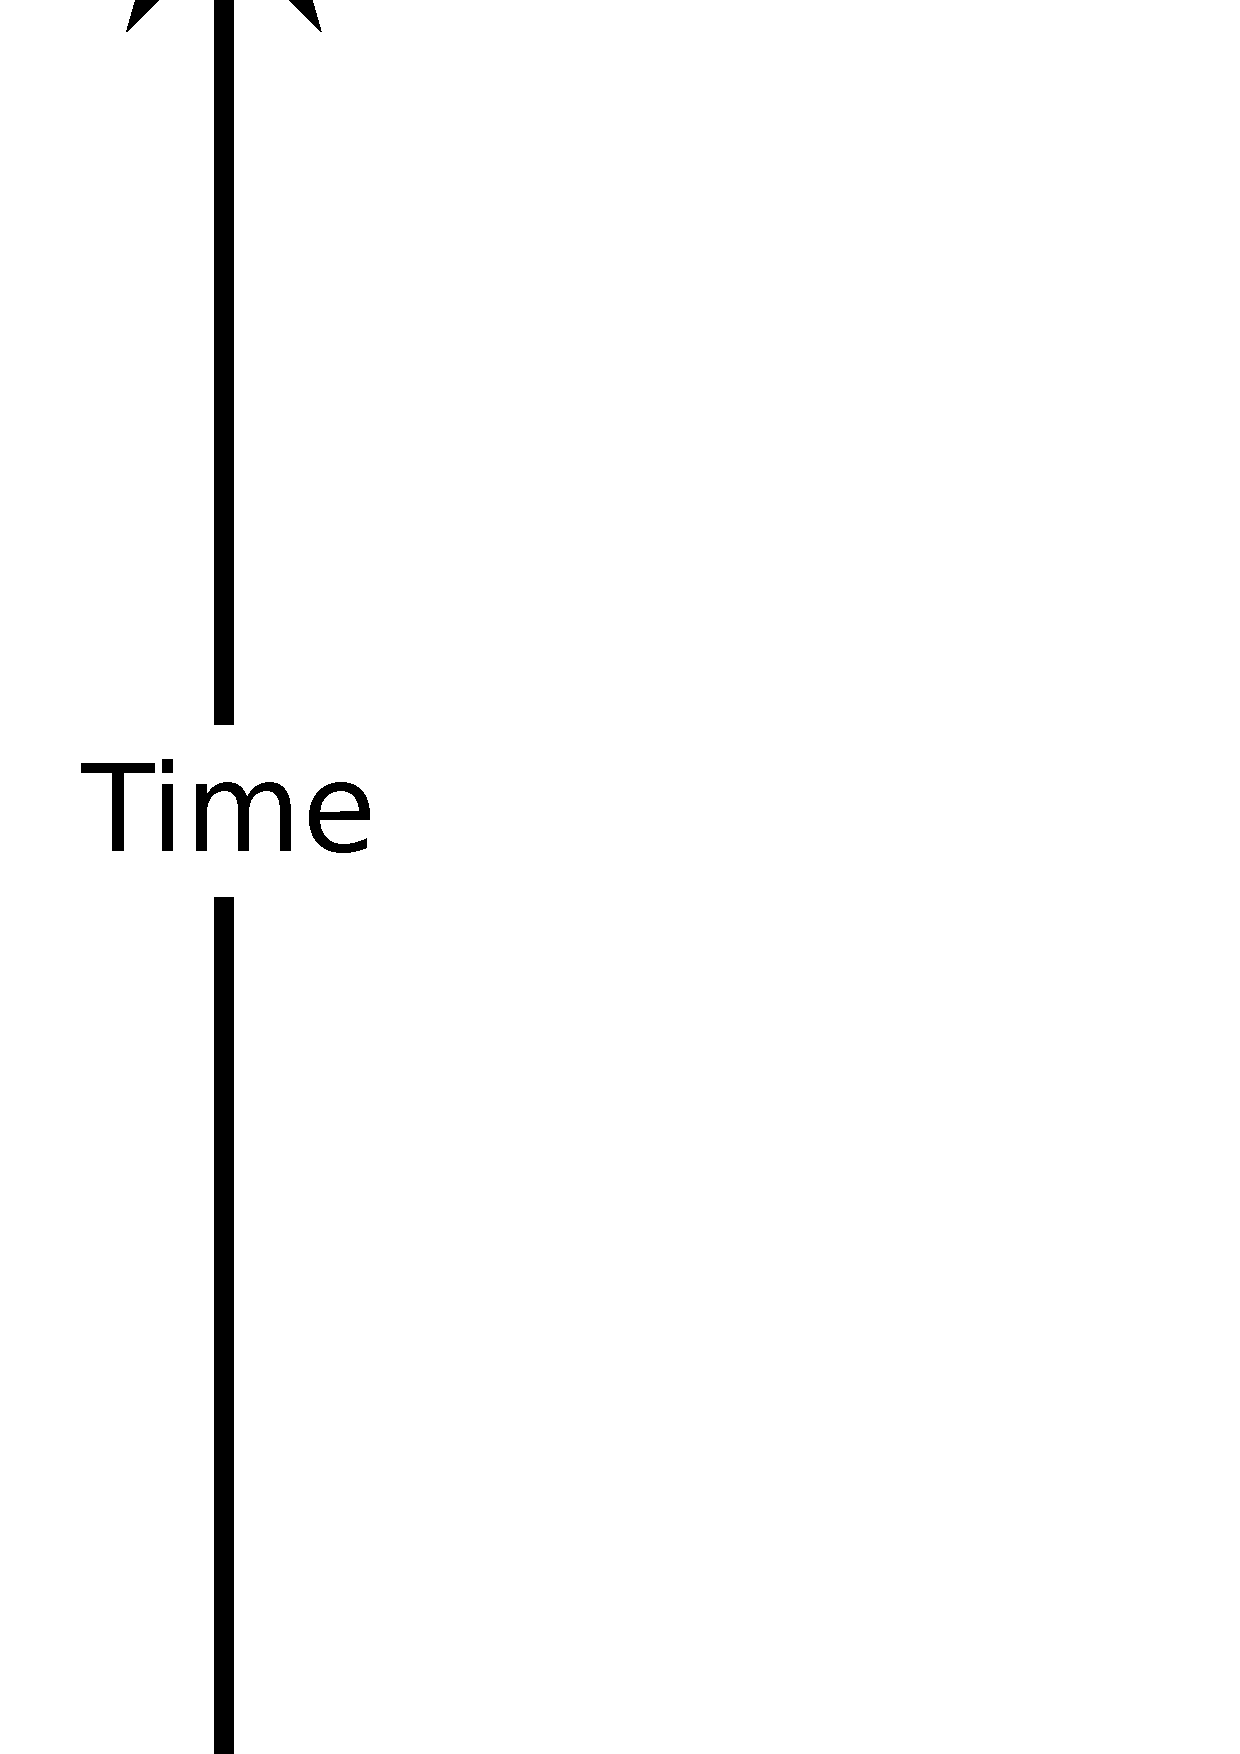
\includegraphics[width=2.5\linewidth]{time.pdf}\\
  \end{minipage}
  \begin{minipage}{0.46\linewidth}
  	\centering
    \scalebox{0.75}{
    \tiny
    \begingroup\makeatletter\def\f@size{1}\check@mathfonts
    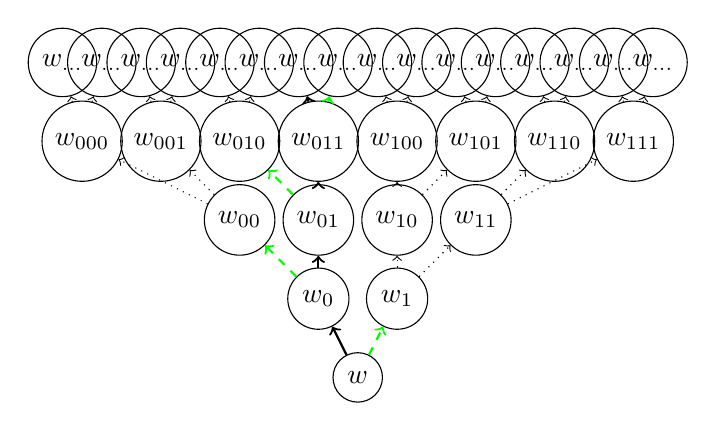
\begin{tikzpicture}
      \node [draw, circle] (w) at (0,0) {$w$};
      \node [draw, circle] (w0) at (-0.5,1) {$w_0$};
      \node [draw, circle] (w1) at (0.5,1) {$w_1$};
      \node [draw, circle] (w00) at (-1.5,2) {$w_{00}$};
      \node [draw, circle] (w01) at (-0.5,2) {$w_{01}$};
      \node [draw, circle] (w10) at (0.5,2) {$w_{10}$};
      \node [draw, circle] (w11) at (1.5,2) {$w_{11}$};
      \node [draw, circle] (w000) at (-3.5,3) {$w_{000}$};
      \node [draw, circle] (w001) at (-2.5,3) {$w_{001}$};
      \node [draw, circle] (w010) at (-1.5,3) {$w_{010}$};
      \node [draw, circle] (w011) at (-0.5,3) {$w_{011}$};
      \node [draw, circle] (w100) at (0.5,3) {$w_{100}$};
      \node [draw, circle] (w101) at (1.5,3) {$w_{101}$};
      \node [draw, circle] (w110) at (2.5,3) {$w_{110}$};
      \node [draw, circle] (w111) at (3.5,3) {$w_{111}$};
      \node [draw, circle] (w0000) at (-3.75,4) {$w_{\dots}$};
      \node [draw, circle] (w0001) at (-3.25,4) {$w_{\dots}$};
      \node [draw, circle] (w0010) at (-2.75,4) {$w_{\dots}$};
      \node [draw, circle] (w0011) at (-2.25,4) {$w_{\dots}$};
      \node [draw, circle] (w0100) at (-1.75,4) {$w_{\dots}$};
      \node [draw, circle] (w0101) at (-1.25,4) {$w_{\dots}$};
      \node [draw, circle] (w0110) at (-0.75,4) {$w_{\dots}$};
      \node [draw, circle] (w0111) at (-0.25,4) {$w_{\dots}$};
      \node [draw, circle] (w1000) at (0.25,4) {$w_{\dots}$};
      \node [draw, circle] (w1001) at (0.75,4) {$w_{\dots}$};
      \node [draw, circle] (w1010) at (1.25,4) {$w_{\dots}$};
      \node [draw, circle] (w1011) at (1.75,4) {$w_{\dots}$};
      \node [draw, circle] (w1100) at (2.25,4) {$w_{\dots}$};
      \node [draw, circle] (w1101) at (2.75,4) {$w_{\dots}$};
      \node [draw, circle] (w1110) at (3.25,4) {$w_{\dots}$};
      \node [draw, circle] (w1111) at (3.75,4) {$w_{\dots}$};
      \draw [thick] [->] (w) to (w0);
      \draw [thick] [dashed] [green] [->] (w) to (w1);
      \draw [thick] [dashed] [green] [->] (w0) to (w00);
      \draw [thick] [->] (w0) to (w01);
      \draw [dotted] [->] (w1) to (w10);
      \draw [dotted] [->] (w1) to (w11);
      \draw [dotted] [->] (w00) to (w000);
      \draw [dotted] [->] (w00) to (w001);
      \draw [thick] [dashed] [green] [->] (w01) to (w010);
      \draw [thick] [->] (w01) to (w011);
      \draw [dotted] [->] (w10) to (w100);
      \draw [dotted] [->] (w10) to (w101);
      \draw [dotted] [->] (w11) to (w110);
      \draw [dotted] [->] (w11) to (w111);
      \draw [dotted] [->] (w000) to (w0000);
      \draw [dotted] [->] (w000) to (w0001);
      \draw [dotted] [->] (w001) to (w0010);
      \draw [dotted] [->] (w001) to (w0011);
      \draw [dotted] [->] (w010) to (w0100);
      \draw [dotted] [->] (w010) to (w0101);
      \draw [thick] [->] (w011) to (w0110);
      \draw [thick] [dashed] [green] [->] (w011) to (w0111);
      \draw [dotted] [->] (w100) to (w1000);
      \draw [dotted] [->] (w100) to (w1001);
      \draw [dotted] [->] (w101) to (w1010);
      \draw [dotted] [->] (w101) to (w1011);
      \draw [dotted] [->] (w110) to (w1100);
      \draw [dotted] [->] (w110) to (w1101);
      \draw [dotted] [->] (w111) to (w1110);
      \draw [dotted] [->] (w111) to (w1111);
      \end{tikzpicture}
      \endgroup
    }\\
    Training with exposure bias
  \end{minipage}
  \begin{minipage}{0.46\linewidth}
  	\centering
    \scalebox{0.75}{
    \tiny
    \begingroup\makeatletter\def\f@size{1}\check@mathfonts
    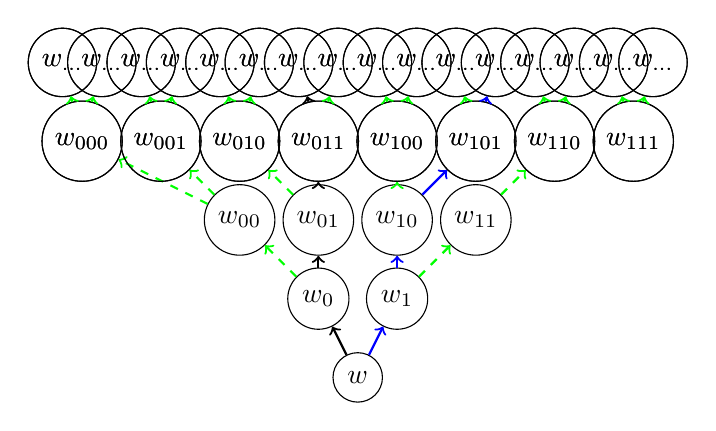
\begin{tikzpicture}
      \node [draw, circle] (w) at (0,0) {$w$};
      \node [draw, circle] (w0) at (-0.5,1) {$w_0$};
      \node [draw, circle] (w1) at (0.5,1) {$w_1$};
      \node [draw, circle] (w00) at (-1.5,2) {$w_{00}$};
      \node [draw, circle] (w01) at (-0.5,2) {$w_{01}$};
      \node [draw, circle] (w10) at (0.5,2) {$w_{10}$};
      \node [draw, circle] (w11) at (1.5,2) {$w_{11}$};
      \node [draw, circle] (w000) at (-3.5,3) {$w_{000}$};
      \node [draw, circle] (w001) at (-2.5,3) {$w_{001}$};
      \node [draw, circle] (w010) at (-1.5,3) {$w_{010}$};
      \node [draw, circle] (w011) at (-0.5,3) {$w_{011}$};
      \node [draw, circle] (w100) at (0.5,3) {$w_{100}$};
      \node [draw, circle] (w101) at (1.5,3) {$w_{101}$};
      \node [draw, circle] (w110) at (2.5,3) {$w_{110}$};
      \node [draw, circle] (w111) at (3.5,3) {$w_{111}$};
      \node [draw, circle] (w0000) at (-3.75,4) {$w_{\dots}$};
      \node [draw, circle] (w0001) at (-3.25,4) {$w_{\dots}$};
      \node [draw, circle] (w0010) at (-2.75,4) {$w_{\dots}$};
      \node [draw, circle] (w0011) at (-2.25,4) {$w_{\dots}$};
      \node [draw, circle] (w0100) at (-1.75,4) {$w_{\dots}$};
      \node [draw, circle] (w0101) at (-1.25,4) {$w_{\dots}$};
      \node [draw, circle] (w0110) at (-0.75,4) {$w_{\dots}$};
      \node [draw, circle] (w0111) at (-0.25,4) {$w_{\dots}$};
      \node [draw, circle] (w1000) at (0.25,4) {$w_{\dots}$};
      \node [draw, circle] (w1001) at (0.75,4) {$w_{\dots}$};
      \node [draw, circle] (w1010) at (1.25,4) {$w_{\dots}$};
      \node [draw, circle] (w1011) at (1.75,4) {$w_{\dots}$};
      \node [draw, circle] (w1100) at (2.25,4) {$w_{\dots}$};
      \node [draw, circle] (w1101) at (2.75,4) {$w_{\dots}$};
      \node [draw, circle] (w1110) at (3.25,4) {$w_{\dots}$};
      \node [draw, circle] (w1111) at (3.75,4) {$w_{\dots}$};

      \draw [thick] [->] (w) to (w0);
      \draw [thick] [blue] [->] (w) to (w1);
      \draw [thick] [dashed] [green] [->] (w0) to (w00);
      \draw [thick] [->] (w0) to (w01);
      \draw [thick] [blue] [->] (w1) to (w10);
      \draw [thick] [dashed] [green] [->] (w1) to (w11);
      \draw [thick] [dashed] [green] [->] (w00) to (w000);
      \draw [thick] [dashed] [green] [->] (w00) to (w001);
      \draw [thick] [dashed] [green] [->] (w01) to (w010);
      \draw [thick] [->] (w01) to (w011);
      \draw [thick] [dashed] [green] [->] (w10) to (w100);
      \draw [thick] [blue] [->] (w10) to (w101);
      \draw [thick] [dashed] [green] [->] (w11) to (w110);
      \node [draw, circle] (w000) at (-3.5,3) {$w_{000}$};
      \node [draw, circle] (w001) at (-2.5,3) {$w_{001}$};
      \node [draw, circle] (w010) at (-1.5,3) {$w_{010}$};
      \node [draw, circle] (w011) at (-0.5,3) {$w_{011}$};
      \node [draw, circle] (w100) at (0.5,3) {$w_{100}$};
      \node [draw, circle] (w101) at (1.5,3) {$w_{101}$};
      \node [draw, circle] (w110) at (2.5,3) {$w_{110}$};
      \node [draw, circle] (w111) at (3.5,3) {$w_{111}$};
      \node [draw, circle] (w0000) at (-3.75,4) {$w_{\dots}$};
      \node [draw, circle] (w0001) at (-3.25,4) {$w_{\dots}$};
      \node [draw, circle] (w0010) at (-2.75,4) {$w_{\dots}$};
      \node [draw, circle] (w0011) at (-2.25,4) {$w_{\dots}$};
      \node [draw, circle] (w0100) at (-1.75,4) {$w_{\dots}$};
      \node [draw, circle] (w0101) at (-1.25,4) {$w_{\dots}$};
      \node [draw, circle] (w0110) at (-0.75,4) {$w_{\dots}$};
      \node [draw, circle] (w0111) at (-0.25,4) {$w_{\dots}$};
      \node [draw, circle] (w1000) at (0.25,4) {$w_{\dots}$};
      \node [draw, circle] (w1001) at (0.75,4) {$w_{\dots}$};
      \node [draw, circle] (w1010) at (1.25,4) {$w_{\dots}$};
      \node [draw, circle] (w1011) at (1.75,4) {$w_{\dots}$};
      \node [draw, circle] (w1100) at (2.25,4) {$w_{\dots}$};
      \node [draw, circle] (w1101) at (2.75,4) {$w_{\dots}$};
      \node [draw, circle] (w1110) at (3.25,4) {$w_{\dots}$};
      \node [draw, circle] (w1111) at (3.75,4) {$w_{\dots}$};
      \draw [thick] [dashed] [green] [->] (w000) to (w0000);
      \draw [thick] [dashed] [green] [->] (w000) to (w0001);
      \draw [thick] [dashed] [green] [->] (w001) to (w0010);
      \draw [thick] [dashed] [green] [->] (w001) to (w0011);
      \draw [thick] [dashed] [green] [->] (w010) to (w0100);
      \draw [thick] [dashed] [green] [->] (w010) to (w0101);
      \draw [thick] [->] (w011) to (w0110);
      \draw [thick] [dashed] [green] [->] (w011) to (w0111);
      \draw [thick] [dashed] [green] [->] (w100) to (w1000);
      \draw [thick] [dashed] [green] [->] (w100) to (w1001);
      \draw [thick] [dashed] [green] [->] (w101) to (w1010);
      \draw [thick] [blue] [->] (w101) to (w1011);
      \draw [thick] [dashed] [green] [->] (w110) to (w1100);
      \draw [thick] [dashed] [green] [->] (w110) to (w1101);
      \draw [thick] [dashed] [green] [->] (w111) to (w1110);
      \draw [thick] [dashed] [green] [->] (w111) to (w1111);
      \end{tikzpicture}
      \endgroup
    }
	Training in expectation (Reinforce)
  \end{minipage}
  \caption{Search space for the toy case of a binary vocabulary and sequences of length 4.  
    The trees represent all the $2^4$ possible sequences.
  The solid black line is the ground truth sequence. 
  \textbf{(Left)} Greedy training such as XENT optimizes only the probability 
  of the next word. The model may consider choices indicated by the green arrows, but it starts off from words taken from the ground truth sequence. The model experiences exposure bias, since it sees only words branching off the ground truth path;
  \textbf{(Right)} REINFORCE and MIXER optimize over all possible sequences, using the predictions made by the model itself.  
  In practice, the model samples only a single path indicated by the blue solid line. The model does not suffer from exposure bias; the model is trained as it is tested.}
  \label{fig:plan}
\end{figure}

  


    


\subsection{The Attentive Encoder}
\label{sup-material:encoder}
Here we explain in detail how we generate the conditioning vector $\bc_t$ 
for our RNN using the source sentence and the current hidden state $\bh_t$. 
Let us denote by $\bs$ the source sentence which is composed of a sequence 
of $M$ words $\bs = [w_1, \ldots, w_M]$. 
With a slight overload of notation let $w_i$ also denote the $d$ dimensional 
learnable embedding of the $i$-th word ($w_i \in \setr^d$). In addition the 
position $i$ of the word $w_i$ is also associated with a learnable embedding $l_i$ 
of size $d$ ($l_i \in \setr^d$). Then the full embedding for 
the $i$-th word in the input sentence is given by $a_i = w_i + l_i$. 
In order for the embeddings to capture local context, we associate an 
aggregate embedding $z_i$ to each word in the source sentence. 
In particular for a word in the $i$-th position, its aggregate embedding 
$z_i$ is computed by taking a window of $q$ consecutive words centered 
at position $i$ and averaging the embeddings of all the words in this window. More precisely, the aggregate embedding $z_i$ is given by: 
\begin{equation}
z_i = \frac{1}{q} \sum_{h = -q/2}^{q/2} a_{i + h}. 
\end{equation}
In our experiments the width $q$ was set to $5$. 
In order to account for the words at the two boundaries of the input 
sentence we first pad the sequence on both sides with dummy words before 
computing the aggregate vectors $z_i$s. Given these aggregate vectors of words, we compute 
the context vector $c_t$ (the final output of the encoder) as: 
\begin{equation}
c_t = \sum_{j=1}^M \alpha_{j,t} w_j, 
\end{equation}
where the weights $\alpha_{j, t}$ are computed as 
\begin{equation}
\alpha_{j, t} = \frac{\exp(z_j \cdot \bh_{t})}{\sum_{i=1}^M \exp(z_i \cdot \bh_{t})}.
\end{equation}



\subsection{Beam Search Algorithm}
\label{sup-material:beam_search}
Equation~\ref{eq:greedy_gen} always chooses the highest scoring next word candidate
at each time step. At test time we can reduce the effect of search error 
by pursuing not only one but $k$ next word candidates at each point, which 
is commonly known as {\it beam search}.
While still approximate, this strategy can recover higher scoring sequences 
that are often also better in terms of our final evaluation metric.
The algorithm maintains the $k$ highest scoring partial
sequences, where $k$ is a hyper-parameter.
Setting $k=1$ reduces the algorithm to a greedy left-to-right search 
(Eq.~\eqref{eq:greedy_gen}). 
%The downside of such an exploration of multiple paths is that it significantly slows down the generation process. The time complexity 
%grows linearly in $k$ because we need to perform $k$ forward passes for our network which is the most time intensive operation. 
%As a result, beam search generation is $k$ times slower than greedy search (Eq.~\eqref{eq:greedy_gen}). 
\begin{algorithm}[!h]
  \KwIn{model $p_{\theta}$, beam size $k$}
  \KwResult{sequence of words $[w_1^g, w_2^g, \dots, w_n^g]$}
  empty heaps $\{\mathcal{H}_t\}_{t = 1, \dots T}$\;
  an empty hidden state vector $\bh_1$\;
  $\mathcal{H}_1.\mbox{push}(1, [[\varnothing], \bh_1])$\;
  \For{$t\leftarrow 1$ \KwTo $T - 1$}{	
    \For{$i\leftarrow 1$ \KwTo $\min(k, \#\mathcal{H}_t)$}{
      $(p, [[w_1, w_2, \dots, w_t], \bh]) \leftarrow \mathcal{H}_t.\mbox{pop}()$\;  
      $\bh' = \phi_\theta(w, \bh)$ \;      
      \For{$w' \leftarrow$ $k$-most likely words $w'$ from $p_\theta(w' | w_t, \bh)$}{
        $p' = p * p_\theta(w' | w, \bh)$\;
        $\mathcal{H}_{t + 1}.\mbox{push}(p', [[w_1, w_2, \dots, w_t, w'], \bh'])$\;
      }
    }
  }
  $(p, [[w_1, w_2, \dots, w_T], \bh]) \leftarrow \mathcal{H}_T.\mbox{pop}()$\;
  \KwOut{$[w_1, w_2, \dots, w_T]$}
 
 \caption{Pseudo-code of beam search with beam size $k$.}
  \label{alg:beam} 
\end{algorithm}


\newpage






\subsection{Notes}
The current version of the paper updates the first version uploaded on arXiv as follows:
\begin{itemize}
\item on the summarization task, we report results using both ROUGE-2 and BLEU to demonstrate that MIXER can work with any metric.
\item on machine translation and image captioning we use LSTM instead of Elman RNN to demonstrate the MIXER can work with any underlying parametric model.
\item BLEU is evaluated using up to 4-grams, and it is computed at the corpus level (except in the image captioning case) as this seems the most common practice
in the summarization and machine translation literature.
\item we have added several references as suggested by our reviewers
\item we have shortened the paper by moving some content to the Supplementary Material. 
\end{itemize}